\problemText{Zanahorias}{Entrada estándar}{Salida estándar}{2 segundos}{}{Dennis Huillca}{FFFFFF}

John trabaja en una empresa llamada "VERDURAS-Tech", y hoy, estaba tan cansado después del trabajo que se quedó dormido en cuanto llegó a casa.Desafortunadamente, incluso en su sueño, no pudo olvidarse de su trabajo. En su sueño, le pidieron que ayudara a una empresa productora de zanahorias con la siguiente pregunta: ¿cuántas zanahorias crecen en un segmento de línea que conecta dos zanahorias dadas? Los extremos del segmento (es decir, las dos zanahorias dadas) no deben incluirse.\\

En su sueño, los representantes de la empresa (gente que tienen zanahorias en lugar de cabezas) dijeron que todas las zanahorias crecen en un plano cartesiano infinito y hay exactamente una zanahoria en cada punto con coordenadas enteras. Debes ayudar al cansado John a resolver este problema.\\

Las coordenadas de las dos zanahorias son $(x1, y1)$ y $(x2, y2)$ respectivamente. Devuelve el número de zanahorias que se encuentran estrictamente en el segmento de línea que conecta estas zanahorias.

\inputText

La primera línea contiene un único número entero $n$ $(1 \le n \le 300)$ indicando el número de casos de prueba.

Las siguientes $n$ líneas contienen cuatro enteros (por línea) $x_1$, $y_1$, $x_2$ y $y_2$ tales que $0 \leq x_1, y_1, x_2, y_2 \leq 50$.

\outputText

Para cada caso de prueba, imprimir el número de zanahorias que se encuentran estrictamente en el segmento de línea que conecta estas dos zanahorias.

% Includes the figures, with the necessary information about your problem
\begin{figure}[h]
  \centering
  \caption{ejemplo para el caso: 1 1 5 5}
  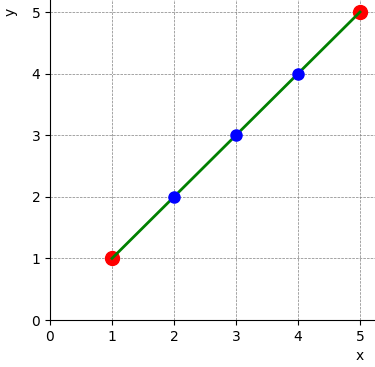
\includegraphics[scale=.5]{2024/Zanahorias/images/zanahorias.png}
\end{figure}

% Command to examples section
\exampleCases

% Create a table with some examples of input and output cases
% Parameters {Example case filepath}
\begin{example}
    \exmp{%%INPUT
        \caseFile{2024/Zanahorias/in/example.in}
    }{%%OUTPUT
        \caseFile{2024/Zanahorias/out/example.out}
    }%%END-OUTPUT
\end{example}